\documentclass[10pt]{article}
\usepackage[polish]{babel}
\usepackage[utf8]{inputenc}
\usepackage[T1]{fontenc}
\usepackage{amsmath}
\usepackage{amsfonts}
\usepackage{amssymb}
\usepackage[version=4]{mhchem}
\usepackage{stmaryrd}
\usepackage{graphicx}
\usepackage[export]{adjustbox}
\graphicspath{ {./images/} }

\title{GIMNAZJUM }

\author{}
\date{}


\newcommand\Varangle{\mathop{{<\!\!\!\!\!\text{\small)}}\:}\nolimits}

\begin{document}
\maketitle
\begin{enumerate}
  \item Punkty \(P\) i \(Q\) leżą odpowiednio na bokach \(B C\) i \(C D\) kwadratu \(A B C D\), przy czym \(B P+D Q=P Q\). Udowodnij, że \(\Varangle Q A P=45^{\circ}\).
  \item Oblicz ile rozwiązań w zależności od parametru \(m\) ma układ równań:
\end{enumerate}

\[
\left\{\begin{array}{c}
|x|+|y|=1 \\
y=|x|+m
\end{array}\right.
\]

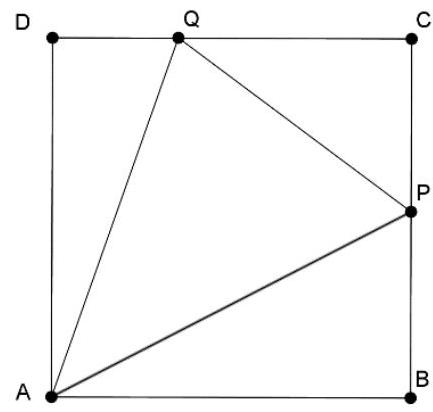
\includegraphics[max width=\textwidth, center]{2024_11_21_cdd85e6b4cedf5476676g-1}\\
3. Rozwiąż w liczbach całkowitych równanie \(x^{2}+y^{2}=2001\)

\section*{LICEUM}
\begin{enumerate}
  \item Na bokach BC i AC trójkąta ABC zbudowano, po jego zewnętrznej stronie kwadraty BCDE i CAFG. Wykaż, że odcinki AD i BG są prostopadłe i równej długości.
  \item Rozwiąż równanie
\end{enumerate}

\[
\left|x^{4}-x\right|+\left|x^{2}-x^{3}\right|=\left|x^{4}-x^{3}+x^{2}-x\right|
\]

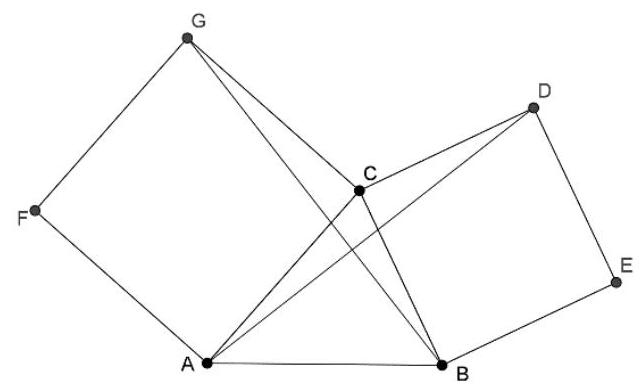
\includegraphics[max width=\textwidth, center]{2024_11_21_cdd85e6b4cedf5476676g-1(1)}\\
3. Rozwiąż w liczbach całkowitych równanie \(x^{2}+y^{2}=2016\)


\end{document}